\section{Experimental Evaluation}
In order to validate our approach, we carry out an extensive and in depth experimental evaluation. As discussed in section \ref{sec:goal}, we study the time-accuracy trade-off. We also do stage-wise analysis where each stage is evaluated independently of others. This helps us understand which stage is acting as bottleneck in terms of performance. Additionally, we also do a noise based analysis to understand the robustness of system to noise. Figure \ref{fig:experimental-methdology} illustrates our experimental evaluation approach graphically. 

\begin{figure}
    \centering
    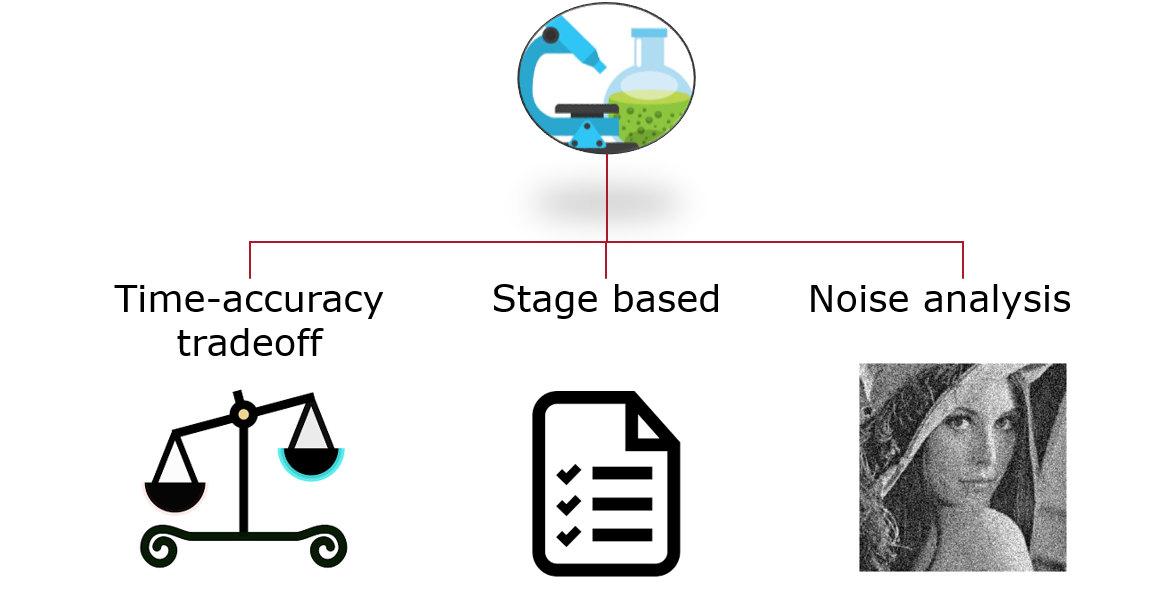
\includegraphics[width=\linewidth]{images/experimental-methdology.PNG}
    \caption{Experimental methodology }
    \label{fig:experimental-methdology}
\end{figure}

\subsection{Dataset}
The dataset we used for experimental evaluation is VIRAT 2.0 \cite{virat20}. It is an outdoor video survillance dataset whose main aim is to facilitate activity classification. It has ground truth annotations of vehicle, person and other arbitrary objects (objects which come in contact with persons during activity). It has approximately 8.5 hours of video data in varying resolution and frames-per-seconds (fps). Figure \ref{fig:virat-samples} shows some samples from the dataset. 

\begin{figure}
    \centering
    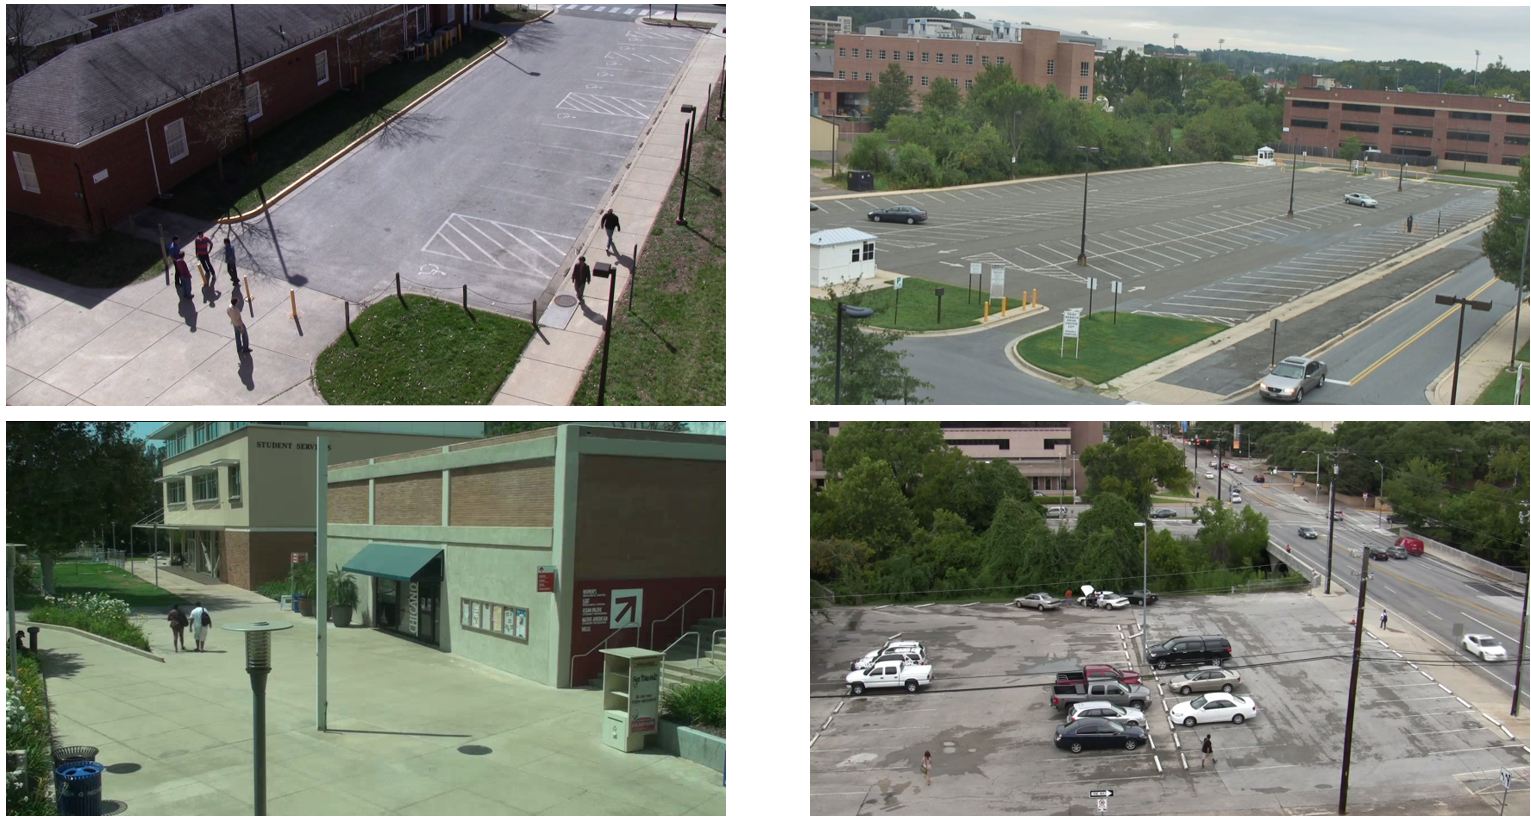
\includegraphics[width=\linewidth]{images/virat-samples.PNG}
    \caption[Samples from VIRAT 2.0 dataset ]{Samples from VIRAT 2.0\cite{virat20} dataset }
    \label{fig:virat-samples}
\end{figure}


\subsubsection{Synthetic dataset}
\label{sec:synthetic-dataset}
Instead of directly using the VIRAT 2.0 dataset, we synthesize more data from it. The reason why we need to do that is original dataset targets activity classification and is therefore enriched with human activity. We on the other hand need sparse activity data. Therefore, we use original VIRAT 2.0 dataset to generate new data that has controlled amount of activity to background ratio. Figure \ref{fig:synthetic-dataset-generator} helps understand our synthetic dataset generator.  

\begin{figure}
    \centering
    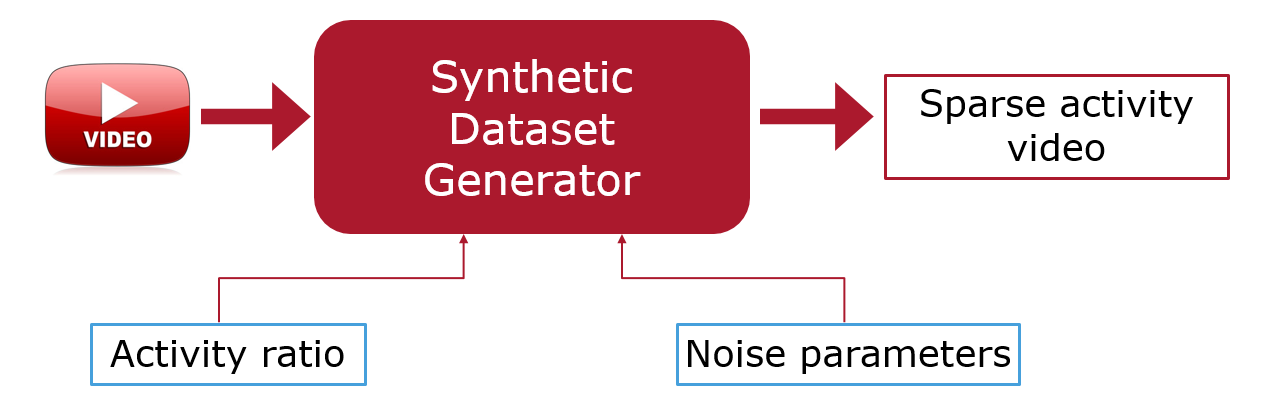
\includegraphics[width=\linewidth]{images/synthetic-dataset-generator.PNG}
    \caption{Synthetic dataset generator}
    \label{fig:synthetic-dataset-generator}
\end{figure}

In order to generate the synthetic data, we follow the following steps:
\begin{enumerate} 
    \item identify background frame
    \item make background block
    \item write background block(s)
    \item write activity block
    \item repeat (3) and (4)
\end{enumerate}

Step 1 is simple. We manually scroll through a video and identify a frame with no activity (ideally no person). In step 2, we repeat the frame $\Delta \times fps$ times where $fps$ is the frame-per-second of original video and $\Delta$ is the target length of background block in seconds. Then we alternatively write background block(s) and activity block in turn. An activity block is simply a section of original video. By default, we use $30s$ long activity blocks. Length of background block is also kept at $30s$ by default. Figure \ref{fig:synthetic-video} helps understand the concept of activity block and synthetic video.  

\begin{figure}
    \centering
    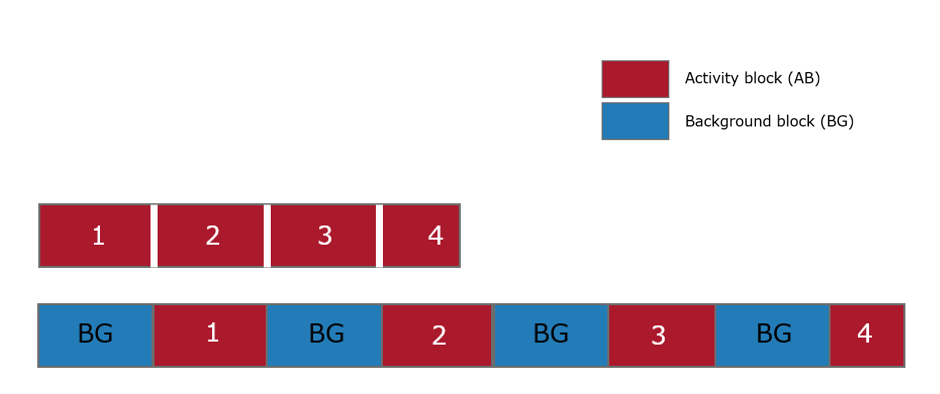
\includegraphics[width=\linewidth]{images/synthetic-video.PNG}
    \caption{Synthetic video illustration}
    \label{fig:synthetic-video}
\end{figure}

An important concept associated with this procedure is \textit{Activity Ratio}. It is defined as 
$$ \text{Activity Ratio} = \text{AR} = \frac{1}{1+nBG} $$
where $nBG=$ no. of background blocks per activity block. Figure \ref{fig:synthetic-video} has $nBG=1$. Table \ref{table:activity-ratio} explains the relationship between $nBG$ and AR. 


\begin{table}
\label{table:activity-ratio}
\caption{Relationship of nBG and AR} \vspace{5pt}
\centering
\begin{tabular}{@{}| l | l | l | @{}} \hline
nBG & nAB:nBG & AR   \\ \hline \hline
1   & 1:1     & 0.5  \\
3   & 1:3     & 0.25 \\
5   & 1:5     & 0.16 \\ \hline
\end{tabular}
\end{table}

\subsubsection{Adding noise}
In order to test the robustness of our approach, we also add noise to our synthetic data. Table \ref{table:noise-params} discuses the parameters that control the level of noise. We use \textbf{salt and pepper} noise in our experiments.

In order to add noise, we first select $p\%$ of frames from each background block. Each of the frame is equally likely to be selected. Now we draw an integer $r$ from normal distribution with parameters $\mu$ and $\sigma$. Now for each selected frame, we select $r$ pixels and add noise to them. Again all pixels are equally likely. 

\begin{table}
\centering
\label{table:noise-params}
\caption{Noise parameters}  \vspace{5pt}
\begin{tabular}{|l|l|}
\hline
parameter & description                              \\ \hline \hline
$p$         & percentage of noisy frames in background block  \\ 
$\mu$        & average no. of noisy pixels in noisy frame     \\ 
$\sigma$     & standard deviation of no. of noisy pixels     \\ \hline
\end{tabular}
\end{table}

\subsection{Evaluation metrics}
We use two performance metrics to measure the performance: f1score and AUC. F1score is selected as a metric to study performance w-r-t detector/classifier threshold. It is useful in the sense that it helps in picking the appropriate threshold for the classifier. AUC on the other hand is independent of a particular threshold. Further, since we are dealing with unbalanced data (background frames may be much more than activity frames); therefore AUC is a more reliable metric for classifier performance as it is insensitive to class imbalance.  
\subsubsection{F1score}
F1score is the harmonic mean of precision and recall. 
$$\frac{1}{f_1} = \frac{0.5}{precision} +  \frac{0.5}{recall} $$
$$precision = \frac{\text{True positive}}{\text{positive predictions}} =  \frac{TP}{TP + FP}$$
$$recall = \frac{\text{True positive}}{\text{actual positives}} =  \frac{TP}{TP + FN}$$

where \\ 
$TP=$ correctly predicted to be positive class\\ 
$FP=$ incorrectly predicted to be positive class\\
$FN=$ incorrectly predicted to be negative class \\

Precision indicates out of samples predicted to be positive, how much is correct! Recall on the other hand indicates how much of the positive samples have been correctly identified. 

\subsubsection{AUC}
AUC stands for Area Under the Curve. It is the area under the TPR-FPR curve (which is also known as Receiver Operating Characteristics (ROC) curve). TPR (True Positive Rate) and FPR (False Positive Rate) are defined as 

$$ TPR = \frac{TP}{TP + FN} = recall$$
$$ FPR = \frac{FP}{FP + TN}$$

A particular value of threshold gives a particular $(FPR,TPR)$ point. This point can be plotted on a 2D plot with TPR on y-axis and FPR on x-axis. Figure \ref{fig:auc} shows a sample ROC curve. As the threshold goes from 0 to 1, the curve moves from top-right to bottom-left. A perfect classifier will have an AUC of 1.0 and a classifier that does no better than random guessing will have an AUC of 0.5. 


\begin{figure}
    \centering
    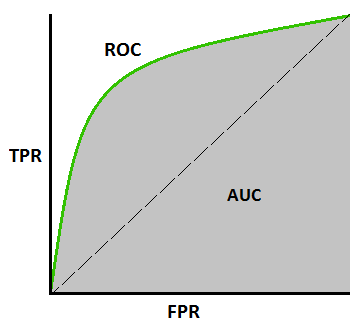
\includegraphics[width=0.6\linewidth]{images/auc.PNG}
    \caption[AUC illustraction]{AUC illustraction. Image taken from \cite{auc}}
    \label{fig:auc}
\end{figure}


\subsection{Time-accuracy trade-off}
In time-accuracy trade off we study how the data can be processed in less time by compromising on accuracy. We vary certain control parameters (stage 1 threshold in this case) and observe time to process the data along with the performance of complete pipeline. Figure \ref{fig:time-acc-tradeoff-mog_vs_gsoc} shows a comparison of MoG and GSoC for the trade off. The trade off curve has f1score on y-axis and normalized processing time on x-axis. Following is the definition of normalized processing time. 
$$\text{normalized time} = \frac{\text{total time to process video data}}{\text{length of video data}}$$
It is clear that as the f1score goes up, the normalized processing time also goes up, indicating the trade off. The figure also shows that MoG significantly outperforms GSoC. For a given f1score, MoG takes less time than GSoC. Alternatively, for a given processing time, MoG shows better performance than GSoC. 

Another interesting fact to note is that it would take around 2.6 hours of normalized processing time to process same data by stage 2 (Faster-RCNN) only. i.e. if stage 1 does not perform filtering. On the other hand, it takes around 1 hour to process the same data using our proposed pipeline.  This shows a 2.6 times improvement in processing time for dataset having AR=0.25. The synthetic dataset parameters using in corresponding dataset are shown in table \ref{table:fig1_data_params}

Figure \ref{fig:time-acc-tradeoff-ar-mog} and \ref{fig:time-acc-tradeoff-ar-gsoc} show similar time-accuracy  trade off for varying activity ratio (AR). For both algorithms, MoG and GSoC, the trade off curve shifts to the left as AR decreases. This is expected as stage 1 can filter more and more frames. Synthetic data parameters are the same as in table \ref{table:fig1_data_params} with the exception of activity ratio. 

\begin{figure}
    \centering
    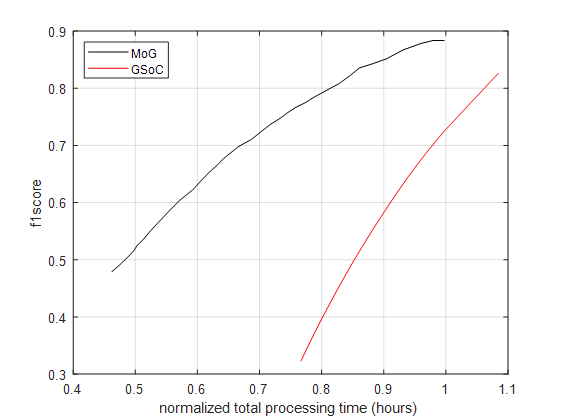
\includegraphics[width=\linewidth]{images/time-acc-tradeoff-mog_vs_gsoc.png}
    \caption[Time-accuracy trade off - MoG vs GSoC]{Time-accuracy trade off - MoG vs GSoC. Synthetic data parameters shown in table \ref{table:fig1_data_params}}
    \label{fig:time-acc-tradeoff-mog_vs_gsoc}
\end{figure}

\begin{table}
\centering
\label{table:fig1_data_params}
\caption{Synthetic data parameters for MoG vs GSoC time-accuracy trade off} \vspace{5pt}
\begin{tabular}{|l|l|}
\hline
parameter             & value  \\ \hline \hline
activity ratio        & 0.25   \\
p                     & 1\%    \\ 
$\mu$    & 0.50\% \\ 
$\sigma$ & 0.20\% \\ \hline
\end{tabular}
\end{table}

\begin{figure}
    \centering
    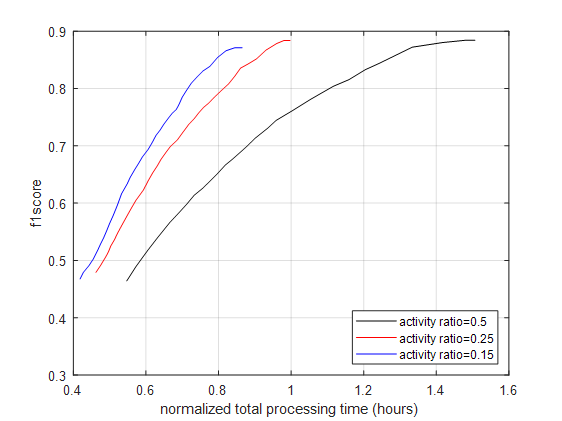
\includegraphics[width=\linewidth]{images/time-acc-tradeoff-ar-mog.png}
    \caption{Time-accuracy trade off for varying AR using MoG}
    \label{fig:time-acc-tradeoff-ar-mog}
\end{figure}

\begin{figure}
    \centering
    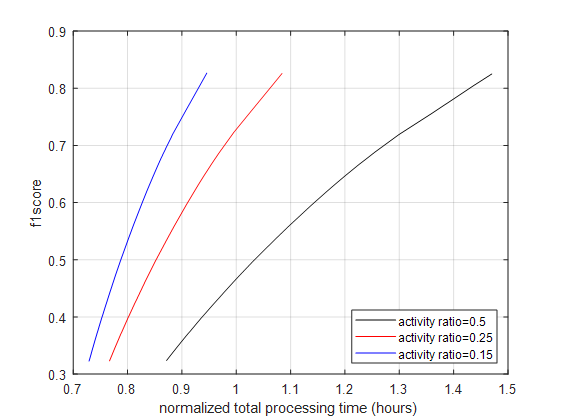
\includegraphics[width=\linewidth]{images/time-acc-tradeoff-ar-gsoc.png}
    \caption{Time-accuracy trade off for varying AR using GSoC}
    \label{fig:time-acc-tradeoff-ar-gsoc}
\end{figure}


\subsection{Stage based }
In this part, we analyse both stage 1 and 2 independently. For stage 1, we are doing binary classification between activity and background frames. We shall vary our threshold (percentage of foreground pixels) and observe f1score. AUC shall also be computed. We will evaluate both MoG and GSoC. Figure \ref{fig:f1-analysis-mog} and \ref{fig:f1-analysis-gsoc} show the results for MoG and GSoC respectively. Table \ref{table:auc-time-analysis-s1} shows the AUC for both algorithms. It is clear that MoG outperform GSoC in both f1score and AUC. Further, MoG is significantly faster as compared to GSoC.   

\begin{figure}
    \centering
    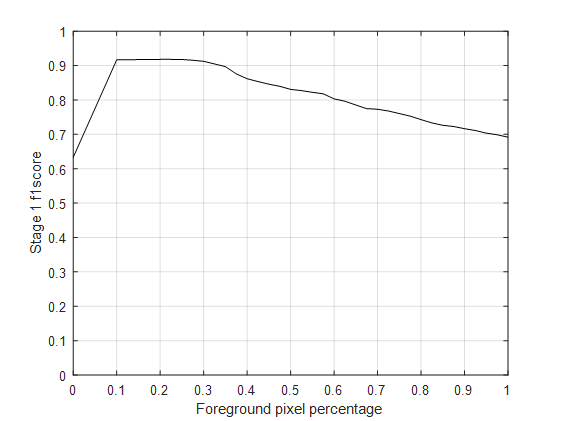
\includegraphics[width=\linewidth]{images/f1-analysis-mog.png}
    \caption{Stage 1 evaluation - MoG}
    \label{fig:f1-analysis-mog}
\end{figure}

\begin{figure}
    \centering
    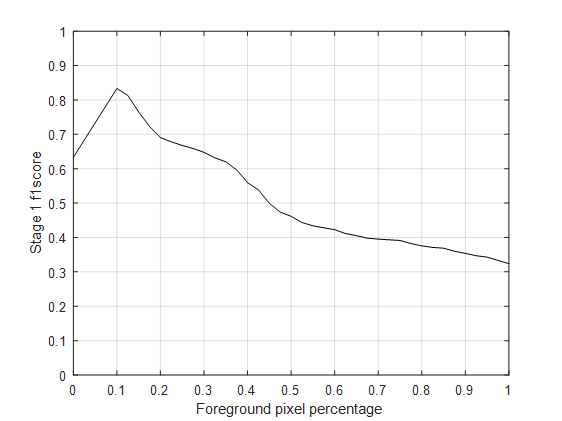
\includegraphics[width=\linewidth]{images/f1-analysis-gsoc.png}
    \caption{Stage 1 evaluation - GSoC}
    \label{fig:f1-analysis-gsoc}
\end{figure}

\begin{table}
\centering
\label{table:auc-time-analysis-s1}
\caption{Stage 1 AUC and time analysis} \vspace{5pt}
\begin{tabular}{|l|l|c|}
\hline
algorithm   & AUC     & mean processing \\
            &         &  time (ms)  \\ \hline \hline
MoG         & 0.94    & 30    \\
GSoC        & 0.6     & 150  \\ \hline
\end{tabular}
\end{table}

For stage 2 evaluation, we adopt a similar methodology. However, we need to clarify how we binarize our predictions. Remember for stage 2

$$
\text{Ground Truth} = 
\begin{cases}
1, &    \text{if there is a person} \\
0, &    \text{otherwise}
\end{cases}
$$

We define the prediction of stage 2 as 
$$
\text{prediction} = 
\begin{cases}
1, &    \text{if there is at least one valid person detection} \\
0, &    \text{otherwise}
\end{cases}
$$

where \\
$\text{valid person detection} = \hat{p}_i>\tau \quad \& \quad IoU(\hat{b}_i,b_j)>0.5$ \\
$\hat{b}_i =i^{th} \text{ prediction bounding box}$ \\
$b_j =j^{th} \text{ ground truth bounding box}$ \\
$\hat{p}_i = i^{th} \text{ prediction probability}$

Based on that, figure \ref{fig:f1-analysis-s2} shows the f1score w-r-t prediction threshold. We achieve an AUC of 0.81 for this stage and we notice that on average it takes 0.5 seconds for the stage 2 (Faster-RCNN) to process one frame at $1080 \times 960$ resolution. 

\begin{figure}
    \centering
    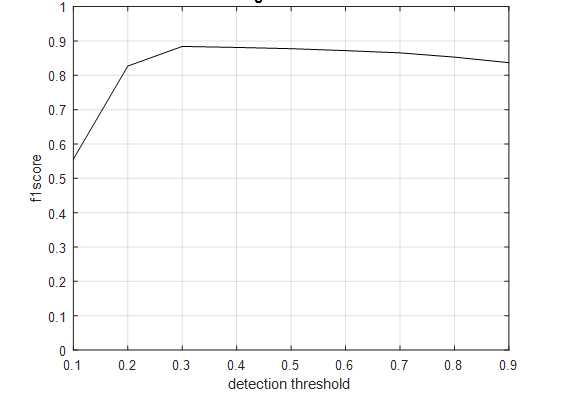
\includegraphics[width=\linewidth]{images/f1-analysis-s2.png}
    \caption{Stage 2 evaluation}
    \label{fig:f1-analysis-s2}
\end{figure}

\subsection{Noise analysis }
Third and final part of our experimental evaluation is noise analysis. In this part, we evaluate the robustness of stage 1 against noise. As discussed in section \ref{sec:synthetic-dataset}, we only add noise to background frames. Noise analysis for stage 2 is not our goal and shall not be discussed here. 

In terms of noise, we have 3 parameters: $p, \mu, \text{ and } \sigma$. Description of these parameters has been discussed in table \ref{table:noise-params}. To study the influence of one parameter, we vary it while keeping the others constant.   

Figure \ref{fig:noise-analysis-mog-p} shows MoG's (stage 1) f1score graph with variation in $p$. We use $AR=0.5$, $\mu=0.5\%$ and $\sigma=0.2\%$ for this experiment. It is clear that increasing the $p$ forces the graph to go down. Thus more noise in terms of $p$ will directly affect the performance of stage 1. This result is also verified by reduced in AUC as shown in table \ref{table:noise-analysis-auc-mog-p}.

Figure \ref{fig:noise-analysis-mog-mu} shows MoG's (stage 1) f1score graph with variation in $\mu$. We use $AR=0.5$, $p=2\%$ and $\sigma=0.2\%$ for this experiment. For variation in $\mu$, the f1score graph again seems to shift downwards for increase in $\mu$. However, the difference is less visible in this case. This result is again verified by reduction in AUC as shown in table \ref{table:noise-analysis-auc-mog-mu}.  

\begin{figure}
    \centering
    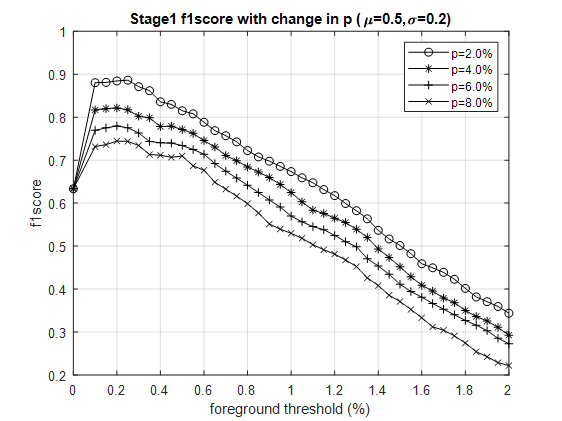
\includegraphics[width=\linewidth]{images/noise-analysis-mog-p.png}
    \caption{Noise analysis - varying $p$}
    \label{fig:noise-analysis-mog-p}
\end{figure}

\begin{figure}
    \centering
    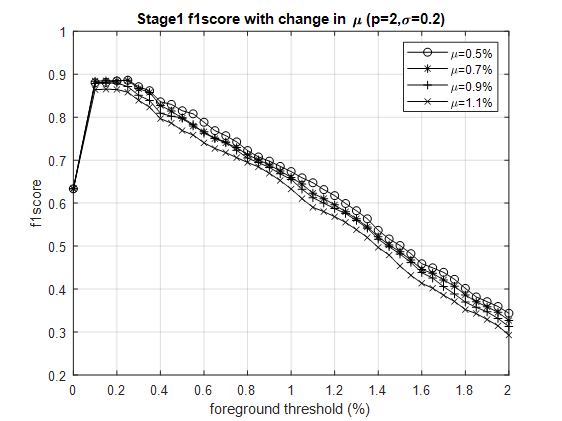
\includegraphics[width=\linewidth]{images/noise-analysis-mog-mu.png}
    \caption{Noise analysis - varying $\mu$}
    \label{fig:noise-analysis-mog-mu}
\end{figure}

\begin{table}
\centering
\label{table:noise-analysis-auc-mog-p}
\caption{Noise analysis - AUC for varying $p$} \vspace{5pt}
\begin{tabular}{|l|l|}
\hline
$p$         & AUC  \\ \hline \hline
2\%         & 0.93   \\
4\%         & 0.87    \\ 
6\%         & 0.83      \\ 
8\%         & 0.78       \\ \hline
\end{tabular}
\end{table}

\begin{table}
\centering
\label{table:noise-analysis-auc-mog-mu}
\caption{Noise analysis - AUC for varying $\mu$} \vspace{5pt}
\begin{tabular}{|l|l|}
\hline
$\mu$         & AUC  \\ \hline \hline
0.5\%         & 0.93   \\
0.7\%         & 0.92    \\ 
0.9\%         & 0.91      \\ 
1.1\%         & 0.88       \\ \hline
\end{tabular}
\end{table}



\newpage